\documentclass{article} % For LaTeX2e
\usepackage{nips13submit_e,times}
\usepackage{hyperref}
\usepackage{url}
\usepackage{amsmath, amsthm, amssymb, mathrsfs}
\usepackage{listings,courier,color}
\usepackage{tikz}
\usepackage[margin=1in]{geometry}
%\documentstyle[nips13submit_09,times,art10]{article} % For LaTeX 2.09


\lstset{language=Matlab}
\lstset{
	basicstyle=\footnotesize\ttfamily,
	breaklines=true,
	morekeywords={assert},
	showstringspaces=false
}
%% definitions.tex
%% @Diao Zheng

%% Contains definitions and shorthands for LaTeX template

% As of v2.2, the following are defined

%\+ : Logical conjunction
%\/ : Logical disjunction
%\! : Logical negation
%\afsoc : Assume for the sake of contradiction
%\amp : Ampersand
%\anf : Arbitrary and fixed
%\band : Conduction of indexed propositions
%\bb{} : Blackboard bold
%\bind{}{} : SML binding
%\bor : Disjunction of indexed propositions
%\ceil{} : Ceiling
%\circled : Circled text
%\code{} : Source code
%\codem{} : Source code in math mode
%\comb{}{} : Combination
%\cov{} : Covariance (matrix)
%\cp : Set compliment
%\D : Set of data
%\dash : Line
%\deriv{} : Derivative
%\derivn{}{} : Nth-order Derivative
%\eqnnum : Numbered equation
%\eqv : Equivalence
%\ev{} : Expected value
%\evc{}{} : Conditional expected value
%\F : False (Contradiction)
%\f : Fourier Transform
%\flr : Floor
%\fr : Fraktur
%\G : Script G
%\imp : Short implication symbol "=>"
%\inv : Inverse (of functions/matrices)
%\mat{} : Contained matrix
%\maxs{} : Maximum of a set
%\mins{} : Minimum of a set
%\mono{} : Monospaced text
%\N : Set of natural numbers
%\n : Set intersection
%\nil : Empty set
%\Nn : Set of natural numbers with zero
%\nn{}{} : Intersection of indexed sets
%\nullity : Nullity of a matrix
%\perm : Permutation
%\pderiv{} : Partial derivative
%\pderivn{}{} : Nth-order partial derivative
%\poly : Set of polynomials
%\prob : Probability
%\ps : Power set
%\R : Set of real numbers
%\rank : Rank of a matrix
%\Rn{} : Rn vector space
%\scr{} : Script
%\set{} : Set builder notation
%\summ{}{} : Summation
%\T : True (Tautology)
%\Tp : Topology
%\Tpb{} : Topology generated by a base
%\tx : Transformation
%\U : Set union
%\UU{}{} : Union of indexed sets
%\var{} : Variance
%\varc{}{} : Conditional variance
%\vc{} : Vector
%\x : Multiplication
%\Z : Set of integers










%augmented matrices
\makeatletter
\renewcommand*\env@matrix[1][*\c@MaxMatrixCols c]{%
  \hskip -\arraycolsep
  \let\@ifnextchar\new@ifnextchar
  \array{#1}}
\makeatother

\newcommand{\deriv}[1]{\frac{d}{d{#1}}}
\newcommand{\pderiv}[1]{\frac{\partial}{\partial {#1}}}
\newcommand{\derivn}[2]{\frac{d^{#2}}{d{#1}^{#2}}}
\newcommand{\pderivn}[2]{\frac{\partial^{#2}}{\partial{#1}^{#2}}}

\newcommand{\R}{\mathbb{R}}
\newcommand{\Rn}[1]{\mathbb{R}^{#1}}
\newcommand{\N}{\mathbb{N}}
\newcommand{\Nn}{\mathbb{N}_0}
\newcommand{\U}{\cup}
\newcommand{\n}{\cap}
\newcommand{\Z}{\mathbb{Z}}
\newcommand{\nil}{\varnothing}
\newcommand{\T}{\top}
\newcommand{\F}{\bot}
\newcommand{\eqv}{\Leftrightarrow}
\newcommand{\UU}[2]{\bigcup^{#2}_{#1}}
\newcommand{\nn}[2]{\bigcap^{#2}_{#1}}
\newcommand{\band}[2]{\bigwedge^{#2}_{#1}}
\newcommand{\bor}[2]{\bigvee^{#2}_{#1}}
\newcommand{\summ}[2]{\sum^{#2}_{#1}}
\newcommand{\poly}{\mathcal{p}}
\newcommand{\bb}{\mathbb}
\newcommand{\scr}{\mathcal}
\newcommand{\fr}{\mathfrak}
\newcommand{\ps}[1]{2^{#1}}
\newcommand{\cp}[1]{{#1}^C}
\newcommand{\f}{\fr{f}}
\newcommand{\amp}{\&}
\newcommand{\imp}{\Rightarrow}
\newcommand{\bmat}{\begin{bmatrix}}
\newcommand{\emat}{\end{bmatrix}}
\newcommand{\vc}{\mathbf}
\newcommand{\x}{\times}
\newcommand{\dash}{\rule[1mm]{10mm}{0.1pt}}
\newcommand{\circled}{\textcircled}
\newcommand{\eqnnum}
           {\stepcounter{eqnno}
             \dash\circled{\theeqnno}}
\newcommand{\+}{\wedge}
\renewcommand{\&}{\wedge}
\renewcommand{\/}{\vee}
\renewcommand{\!}{\neg}
\newcommand{\inv}[1]{{#1}^{-1}}
\newcommand{\tx}[1]{xrightarrow{#1}}
\newcommand{\Tp}{\scr{T}}
\newcommand{\set}[1]{\{#1\}}
\newcommand{\afsoc}{Assume for the sake of contradiction}
\newcommand{\anf}{arbitrary and fixed}
\newcommand{\Tpb}[1]{\Tp_{\scr{#1}}}
\newcommand{\maxs}[1]{\text{max }\{#1\}}
\newcommand{\mins}[1]{\text{min }\{#1\}}
\newcommand{\rank}{\text{rank}}
\newcommand{\nullity}{\text{nullity}}
\newcommand{\flr}[1]{\lfloor{#1}\rfloor}
\newcommand{\ceil}[1]{\lceil{#1}\rceil}
\newcommand{\code}[1]{\lstinline$#1$}
\newcommand{\codem}[1]{\text{\lstinline|#1|}}
\newcommand{\mono}[1]{\lstinline[keywordstyle={}]|#1|}
\newcommand{\bind}[2]{[\code{#1}/\code{#2}]}
\newcommand{\D}{\scr{D}}
\newcommand{\nCr}{\binom}
\newcommand{\perm}[2]{\,^{#1}P_{#2}}
\newcommand{\ev}[1]{\vc{E}[{#1}]}
\newcommand{\evc}[2]{\vc{E}_{#1}[{#2}]}
\newcommand{\var}[1]{\text{Var}[{#1}]}
\newcommand{\varc}[2]{\text{Var}_{#1}[{#2}]}
\newcommand{\cov}[1]{\vc{Cov}[{#1}]}
\newcommand{\prob}[1]{\vc{Pr}[{#1}]}
\newcommand{\comb}[2]{{{#1} \choose {#2}}}
\newcommand{\defeq}{\mathrel{\overset{\makebox[0pt]{\mbox{\normalfont\tiny\sffamily def}}}{=}}}



\title{10-601 Final Project Midway Report}


\author{
Simon Diao\\
Carnegie Mellon University\\
Pittsburgh, PA 15213 \\
\texttt{zdiao@andrew.cmu.edu} \\
\And
Nicolas Badoux \\
\'Ecole Polytechnique F\'ed\'erale de Lausanne \\
Switzerland \\
\texttt{nbadoux@andrew.cmu.edu} \\
}

% The \author macro works with any number of authors. There are two commands
% used to separate the names and addresses of multiple authors: \And and \AND.
%
% Using \And between authors leaves it to \LaTeX{} to determine where to break
% the lines. Using \AND forces a linebreak at that point. So, if \LaTeX{}
% puts 3 of 4 authors names on the first line, and the last on the second
% line, try using \AND instead of \And before the third author name.

\newcommand{\fix}{\marginpar{FIX}}
\newcommand{\new}{\marginpar{NEW}}

\nipsfinalcopy % Uncomment for camera-ready version

\begin{document}


\maketitle

\begin{abstract}
In this final report, we managed to use 3 different classifiers, a $k$th nearest neighbour, a neural network classifier and logistic regression classifier to achieve a reasonable classification accuracy of a subset of CIFAR-10 images dubbed \code{subset_CIFAR10}. We also implemented classifiers such as na\"ive Bayes decision tree with little success. We have also investigated different features to use in classification.
\end{abstract}

\section{Introduction}

For this project, we aim to classify CIFAR-10 images dataset - a collection of 10000 32$\x$32 pixels images, into one of ten categories. As per project requirements,
our classifiers are trained solely on a subset of 5000 CIFAR-10 images provided to us as \code{subset_CIFAR10}. As of the date of the final report, we have explored many
classifiers, including Na\"ive Bayes, logistic regression, neural network, deep neural network, convolutional neural network, decision tree, and $k$th nearest neighbour. 
In comparison the our advancement at the midway report, we managed to improve our neural network to a decent accuracy and speed up our $k$th nearest neighbour enough so that it complete in the 10 minutes times frame allowed on Autolab.  We were also able to implement a classifier in an above baseline accuracy using Logistic Regression.

\subsection{Motivation}

We decided to focus primarily on neural networks due to its ability to model many abstract concepts, and neural networks, especially convolution neural networks (CNN), such as LeNet,
has seen great success in the area of image recognition. Our goal for this project is to implement a working CNN to classify the given dataset. However, in doing so, we would have 
to face many challenges, including initialisation of values, performing back-propagation on convolutional and pooling layers, and find the optimal set of parameters for optimal
performance.

\subsection{Background and Related Work}

Xavier Glorot and Yoshua Bengio [1] noted that initialisation of neural network weights should be sampled from a distribution of mean 0 and variance $\frac{2}{n_{in}+n_{out}}$.
Further research was done in attempt to understand convolutional neural networks in terms of concept and implementation. Heaton noted that the following was to be considered when determining the size of hidden layers in a neural network [2]:
\begin{itemize}
  \item The number of hidden neurons should be between the size of the input layer and the size of the output layer.
  \item The number of hidden neurons should be 2/3 the size of the input layer, plus the size of the output layer.
  \item The number of hidden neurons should be less than twice the size of the input layer.
\end{itemize}

\subsection{Dataset}
CIFAR-10 is a labeled subset of the 80 million tiny images [4]. The training data is a random subset of CIFAR-10 which contains 5000 labeled color images (size of 32*32*3) balanced in 10 different classes, while the test set is a random subset of an unknown number of images without disclosure of their labels. After the classification model is well trained with appropriate parameters, it will be used for testing set in order to generate predicting labels. Below is a random sample from the CIFAR-10 with 10 random images from each class [4].

\begin{figure}
\centering
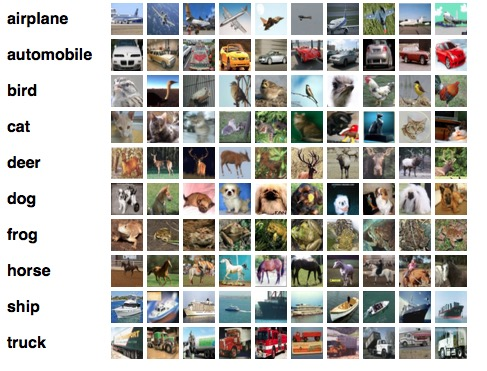
\includegraphics[scale=0.55]{data.jpg}
\caption{A sample of images in 10 different classes. }
\end{figure}


\section{Method}
Methodology is further broken down into three parts, classifiers, feature selection and training.




\subsection{Classifiers}
We have attempted and tried various supervised learning algorithms, some with more success than others.

\subsubsection{Na\"ive Bayes}
The Na\"ive Bayes classifier seeks to maximise
$$\prob{Y|X}$$
with the assumption that
$$\forall i,j,  i\neq j \cdot \prob{X_i|X_j, Y}=\prob{X_i|Y}$$
In other words, it assumes that all input features are conditionally independent of each other given the prior. However, in the case of image classification, this assumption does
not hold very well, as in a normal image, the intensity or colour of a pixel will depend on the intensities and colours of neighbouring pixels. Therefore, using raw pixel values (both 
RGB and HSV\footnote{Hue, Saturation and Value. This colour space separates the hue, or colour from its intensity and brightness, and we can treat the three values as essentially independent of each other.}), we were only able to achieve around $30\%$ classification accuracy. Using histogram of oriented gradients improved the classification accuracy to $48.7\%$. However, we
were unable to improve on the classification accuracy. We did attempt to change the \code{cell_size} parameter, however, we found that at higher values, it leads to overfitting, and
at lower levels, it reduces classification accuracy.

The classifier was implemented as Gaussian features each with a mean and variance estimate. Log likelihood was used to avoid floating-point underflow. However, other posterior distributions could also be considered, such as Beta in case of pixel values.

\subsubsection{Neural Network}
Most of our time was focused on attempting to produce a useable classifier using a neural network. We implemented three variants of neural networks, a simple neural network with 1 hidden layer, a deep neural network with multiple hidden layers of the same size, and a convolutional neural network with one convolutional layer, one pooling layer and a fully connected layer.

For all of our neural network layers (other than the convolutional and pooling layers), the activation function is given as

$$o = \frac{1}{1+e^{-X\cdot W}}$$

where $o$ is the output, and $X$ is the input layer and $W$ is the associated weight, which we then initialised using Xavier initialisation discussed earlier and trained using back-propagation.
We also used entropy as objective function, where
$$\delta_k = o_k(1-o_k)(t_k-o_k)$$
where $t_k$ is the expected output of the $k$th neuron. Furthermore, for all of our neural network implementations, the final layer had 10 neurons, each indicating a class probability. The final decision is reached by 
$$\arg\max_k o_k$$

In order to visualise the gradient descent, we implemented two error functions:
  $$E_1 = \summ{i}{}{|t_i-o_i|}$$
and
  $$E_2 = \summ{i}{}{(t_i-o_i)^2}$$
Both these errors were only used once per epoch to test for convergence, which we defined as $E_{t}\geq E_{t-1}$.

\begin{figure}
\centering
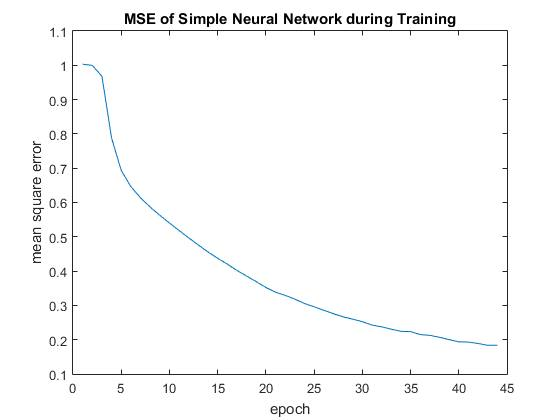
\includegraphics[scale=0.55]{MSENN.jpg}
\caption{Evolution of the error ($E_2$) during training. }
\end{figure}


The final classifier we decided to implement consists of 496 input layers, each corresponding to a HOG feature (with a cell size of 8), 236 hidden layers and 10 output layers. The activation function for each of the hidden layers is as follows:
  $$o = \frac{1}{1+e^{-(x\cdot w+b)}}$$
where $w$ is the weight given to any of the $x$s, and $b$ is a scalar that indicate the bias of this neuron. Both $w$ and $b$ are learnt by stochastic gradient descent. with a learning rate $\eta=0.001$ and momentum $\alpha=0.8$.


\subsubsection{$k$th Nearest Neighbour}
Our final attempt at a classifier was to implement $k$th nearest neighbour with a image kernel. $k$th nearest neighbour seeks to find the, as the name suggest, $k$ nearest neighbours and obtain the mode label. We have tried a variety of input features with this algorithm, including dominant colour, scale-invariant feature transform (SIFT), and histogram of oriented gradients (HOG). For SIFT, the distance metric was to first perform \code{vl_ubcmatch} on test sample and neighbour, and order neighbours by number of matches and then by sum of distance, so suppose that
\begin{lstlisting}
  [~, scores] = vl_ubcmatch(sample, neighbour);
  [n, d] = size(scores);
\end{lstlisting}
then
$$A < B \eqv \codem{n}_A>\codem{n}_B \/ (\codem{n}_A=\codem{n}_B\+\summ{i=0}{\codem{n}_A}{\codem{scores}_{A,i}}<\summ{i=0}{\codem{n}_B}{\codem{scores}_{B,i}})$$

However, this metric did not perform very well, and its classification accuracy was around $30\%$.

We also used HOG features with $\codem{cell_size}=8$. Here, our distance metric is the L1 sum of the difference of the HOG features. Suppose that the HOG feature of each image is a $N\x N\x K$ tensor, and the HOG features of the test image and its neighbour is $F$ and $G$ respectively, then our distance metric can be characterised as
$$d=\summ{i=1}{N}\summ{j=1}{N}\summ{k=1}{K}|F_{ijk}-G_{ijk}|$$

For the midway report, we were not able to respect the maximum of running time of 10 minutes. For this report we were able to improve our running time and therefore fit in the time window of Autolab. Sadly, we had to reduce the size of the training set, reducing therefore our accuracy. Our accuracy is now of $49.1\%$ instead of the 53\% advertised in the midway report.

Our improvements for  $k$ nearest neighbour consist mostly of implementing a datastructure known as $kd$-tree (k-dimensional tree). This datastructure is a space partitioning datastructure. It is similar in the form to a binary tree. Each node that is not part of the leafs represent an hyperplane in a particular dimension cutting a subspace in two. Each level of the $kd$-tree is another dimension above the previous one. The root level representing dimension one. Since we use hog, our data still have a really high number of features and we don't use each feature as a dimension. 


The interest of $kd$-tree come from the fact that while searching for the $k$ nearest neighbour, the datastructure let us discard half the points if the distance between the actual furthest neighbour and the point is smaller than the distance from the hyperplane to the point. The justification is easy to see on a figure: if the furthest neighbour actually found is on the same side of the hyperplane than the point, there is no need to look at the other side of the hyperplane (see Figure 3.).
\begin{figure}
\centering
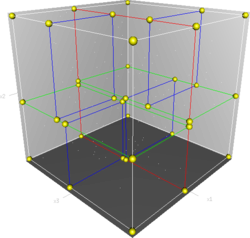
\includegraphics[scale=0.8]{3dtree.png}
\caption{Representation of a $3$d-tree. First split in red, second in green and third in blue. [5]}
\end{figure}
Because the relative slow classification come form the number of comparison to do between each points to find the nearest neighbours, being able to reduce the size of the set of points is an interesting speed up. The implementation of the $kd$-tree is done using the \code{struct} elements in Matlab. 

Although in theory, we reduce the running time from $\mathcal{O}(f*N)$ where f is the number of features and N the number of points to $\mathcal{O}(\log{}N)$, our speed up is smaller due to a perfectible implementation, the use of \code{struct} instead of our own datastructure and points not uniformly placed . Our speedup is around $30$\%.
We also had to implement a bounded priority queue keep track of the nearest neighbours effectively. This priority queue was implemented using a normal Matlab array.




\subsubsection{Deep Neural Network}

The last classifier we used is a Deep Neural Network. A Deep Neural Network or DDN for short is a neural network with multiple layers allowing this way to model and classify more abstract data. 

As for Neural Netwrok, we used the $L_2$ error to test our convergence.
 $$L_2 = \summ{i}{}{(t_i-o_i)^2}$$

One trick that we used to train our Deep Neural Network is Learning rate decay. Decreasing the learning rate trough time help us in multiple way. First, if the learning rate is constant and big, we will never converge. Conversely, if the learning rate it too small, we can get stuck in a local minima in addition to the fact that the learning will be really slow. Using a learning rate depending on the iteration number let us counter this two risks.
As recommend by Samy Bengio [3], we used this decay function:

$$\eta(s)=\dfrac{\eta_0}{(1+\eta_d*s)}$$ 
where $\eta_0$ is the initial learning rate and $\eta_d$ is the rate at which the learning rate decay. 
We choose an $\eta_0 = 1$ and an $\eta_d = 0.1$.

For this classifier we ended up choosing to use 3 hidden layers, each composed respectively of $374, 253, 131$ neurons. The output layer output the number of class and therefore contains 10 neurons. The input layer is composed of 496 layers since we used a size of cell of 8 in the computation of the HOG value. 

\begin{figure}
\centering
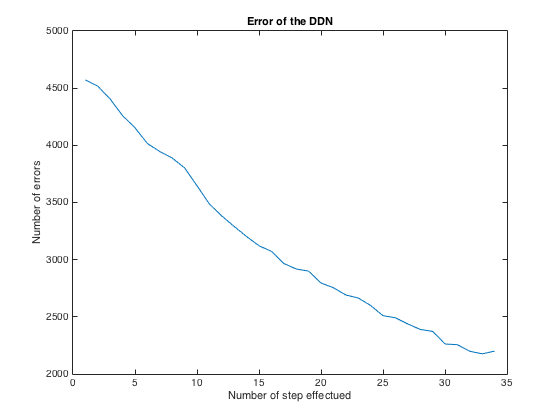
\includegraphics[scale=0.55]{ErrorDNN.png}
\caption{Evolution of the number of error on a dataset of 5000 images until the DNN reach convergence. }
\end{figure}

Our classifier converges in approximately 35 steps with an $L_2$ error in the region of $45\%$.

\subsection{Features Extraction}
We have attempted to extract different features from the image in order to reduce noise in the data.

\subsubsection{Raw Pixel Data}
We have trained some classifier with the raw pixel value, both RGB, HSV and intensity. Until now we did not get a good result. However, we are hopeful that a well-trained convolutional neural network would be able to produce reasonable results with raw pixel values.

\subsubsection{Dominant Colour}
We noticed that some colours in the image only appears on specific classes, such as red, thus we theorised that dominant colours could aid us in classification. To obtain it, we applied a blur to the image to smooth the colour. To extract the dominant color, we sampled the image every 4 pixels and compared the colour sampled to every pixel in the image, counting how many pixels are in a certain range of the sampled color.

We sample every four pixels to spare some computations. Since we are trying to find the dominant colour, it's quite certain that even looking to only one fourth of the pixel we will encounter the most dominant colour. We also check that the colour picked is not the already dominant colour. The range is 100 and is the sum of the differences between the R, G and B values. 

Sadly, we didn't had time to optimize this feature detection enough so that it run in a decent time. Therefore we were not able to use it on Autolab for the submission of this report.

\subsubsection{Edge detection}
We apply a simple Sobel algorithm on the grayscale image. We have also implemented an edge detection on the different R, G and B channels and then regroup the different edges. This give us an interesting result, some edges appear only in some color channel (like between a blue sky and a blue sea, the blue channel would not give us any result but the red channel can). Comparing it with the grayscale edge detection give also some feedback.

\subsubsection{Horizontal Line}

We also tried to find an horizontal edge in the image. This could mean an horizon (like in the case of a ship at sea) or a straight horizontal line (for example a photo of a truck sideways). To extract this feature, we first applied the Sobel algorithm to the image with reasonable threshold (0.14 in this case). Then we went trough the lines of the image and counted how many pixel were on the line, just above or just below and are marked as edges. A higher number represent lot of edges in the same horizontal area. 

To counter the case were we would just had a lot of edges but not specially in a horizontal shape and not give a higher score with an image with fewer pixel marked as edges but all in an horizontal line, we subtract to the highest number we found, the 4th highest number. That means, we take the group of 3 lines with the maximum of pixel denoted as edges and decrease this value by the number of pixel denoted as edges in another group of 3 lines. Therefore, if the image has lot of pixel marked as edges but not particularly in a horizontal line, the score would be much nearer to zero. 

\subsubsection{Histogram of Oriented Gradients}
We have also used VLFeat to extract the Histogram of oriented gradients (HOG).
We are still trying to adjust the cell size to match at best our classifier without timing out. 
The HOG values give us some insight on the edges as well as on color or intensity value of the image. Therefore it's a quite interesting feature that gave us some good result alone. 

\subsection{Training}
We have also attempted various methods of training the different classifiers. For Na\"ive Bayes, we used MLE log likelihood with Gaussian likelihoods. However, if we were to use feature values that which are bounded in one end or two, other distributions, such as Gamma or Beta could prove to be more useful. We could also use semi-supervised learning and boosting to boost the performance of Na\"ive Bayes classifier.

\section{Experiments and Results}

\subsection{Selection of Hidden Units in Neural Network}

Our neural network classifier design used 496 input neurons as the result of a HOG feature with cell size 8, and 10 output neurons each representing the probability of classifying the image into one of the classes. The class picked is the class label with the highest probability, i.e. $\arg\max_i {x_i}$. To determine the optimal number of neurons in the hidden layer, we conformed to Heaton's suggestions [2] and trained 3 neural networks each with a number of hidden neurons ranging from 200 to 300, resulting in 300 different networks. Each of the networks is trained with a learning rate $\eta=0.001$ and momentum $\alpha=0.8$. For each network, we computed the training accuracy and test accuracy. Training accuracy was achieved by running the classifier on the 5000 given training samples, whereas test accuracy was achieved using the 10000-image \code{test_batch} in the CIFAR-10 dataset. We then plotted the $\max$ of both training and test accuracy\footnote{The classifiers with the $\max$ training and test accuracies are not necessarily the same ones.}. The results are shown in Figure 5. We have seen that the test accuracy is relatively consistent when the number of hidden neurons is between 200 to 260, however, as the number of neurons increases above 290, the chances for gradient descent to find a local minimum that is giving a baseline reading of 0.1\footnote{This baseline is simply classifying everything as one class (i.e. picking the most popular class label).} increases. However, it could also be that we are extremely unlucky in our simulation where none of the 3 initialisations gives the optimal result. running Matlab's \code{max} function on test accuracy gives the number of hidden neurons to be 236, which is the value we used as hidden layer. We noticed that for non-baseline classifiers, the training accuracy is significantly higher than test accuracy, and the training accuracy also fluctuates much greater than test accuracy. Hence, we conclude that a hidden layer of anywhere between 200-260 neurons could be optimal for our network.

\begin{figure}
\centering
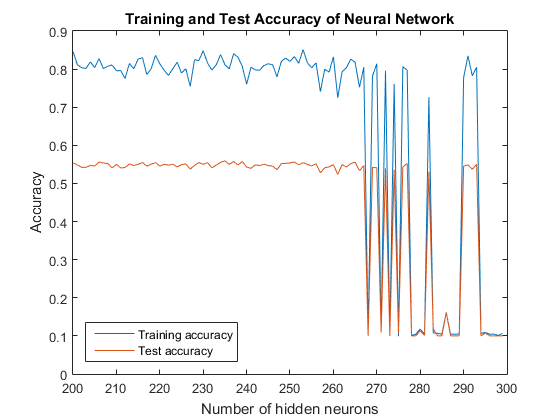
\includegraphics[scale=0.65]{fig1.png}
\caption{The training and test errors for our neural network.}
\end{figure}

\subsection{Choosing $k$ in $k$-Nearest Neighbour}

The choice of $k$ in $k$ th nearest neighbour is an important point for this algorithm. A small k, means our algorithm will be much more influenced by noise or small variation in the data. Conversely, a big $k$ will not be much influenced by the noise but also weaken our hypothesis that points near each other have the same labels. In addition to that, a bigger $k$ will slow down our algorithm since we will have to look at more neighbours before being able to use the properties of our $kd$ tree. A widely spread rule of thumb on internet and in the literature is that  $\sqrt[2]{N}$ (where N is the number of class) is a good choice but not always optimal. 
We have experimented our $k$ nearest neighbour algorithm with different value of $k$ using leave-one-out cross validation. As we can see in Figure 6. The optimal k for our dataset $k$ is around 7. 
We can clearly see a increase in the error rate when we have a much higher $k$ meaning that we include a too big region and some points in the border will be misclassified. 


\begin{figure}
\centering
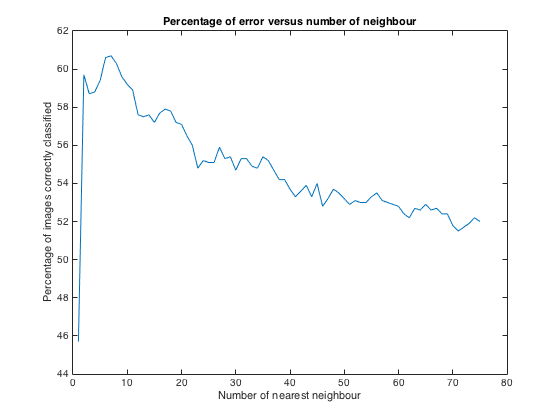
\includegraphics[scale=0.5]{kChoice.png}
\caption{The number of neighbour and the test error. }
\end{figure}






\section{Conclusion and Further Improvements}

Even if we are far from the smallest error rate achieved in the literature or in the class, we were able to fulfill the requirements of this project. Even if it was not always easy and  we went trough a lot of different classifiers, we were able to achieve above baseline ($48.7\%$) classification for three of them.

Our classifiers endured important changes and improvements since from the midway report. We went from having only one classifier working too slowly, to three fully functional decent classifiers.

The use of a special datastructure for $k$ nearest neighbour was necessary and brought the speed-up expected. Even with this improvement, $k$ nearest neighbour is still very slow for the classification in comparison to other classifiers. Therefore, if we need to classify regularly new images or a higher number of images, we would investigate some other classifiers.

We didn't spend a lot of time trying to counter overfitting. This would probably be an interesting track to follow to improve even more our classifiers. 

Our features extractions were usable but far from excellent. It was difficult to assign a good output value, consistent with the other features. The use of VLFeat really helped and if we would had to improve our project further we would look to more complex features extraction reposing on strong theory basis. 

One of our failure was bringing convolutionnal neural network to work completely. Even with the long time we spent working on this classifier we were not able to find the combination of parameters to get a decent result. We are confident that with more time we would have brought this classifier to work and probably achieved a really good score as other implementations testifies.

We would have like to improve our Deep Neural Network by replacing the output layer that just take the maximum by a Support Vector Machine or a Mixture Model. 




\section{References}
\small{
[1] Glorot, X., \& Bengio, Y. (2010). Understanding the difficulty of training deep feedforward neural networks. \textit{In International conference on artificial intelligence and statistics} (pp. 249-256).

[2] Heaton, J. (2008). \textit{Introduction to Neural Networks for Java} (2nd ed., pp. 158-159). St. Louis, Mo.: Heaton research.


[3] Bengio, S. (2003). \textit{An Introduction to Statistical Machine Learning - Neural Networks -} (slides 32) Martigny, CH.: Dalle Molle Institute for Perceptual Artificial Intelligence (IDIAP)

[4] Alex, K. (2009). \textit{Learning multiple layers of features from tiny images}

[5] Wikimedia.org. \url{https://commons.wikimedia.org/wiki/File:3dtree.png}
}


\end{document}
